%!TEX root = main.tex
\chapter{Pose Estimation}\label{chapter:Pose Estimation}
\section{Overview}
As already was mentioned in introduction, estimating the pose (sometimes says tracking) of camera is a crucial part in most of computer vision applications. In the case of augmented reality applications, currently two approaches have been used: marker-based pose estimation and feature-based pose estimation. In both approaches, the pose estimator try to make an estimation of camera relative to the scene. For both approaches, there are so many techniques that were explained in previous sections. Ubitrack framework is an open source library for augmented reality that is developed by FAR group in TUM. The marker-based pose estimation approach already was added to Ubitrack by Sven Barth \cite{barth2014marker}. This method that was inspired by PTAM \cite{klein2007parallel}, detect the corners of all markers and estimates the pose of camera by using tracking and mapping tasks.\\
The main point of this thesis is to add one efficient and precise feature-based pose estimation approach to the Ubitrack framework. To reach to this point, some requirement algorithms such as robust feature matching and bundle adjustment were developed and added to Ubitrack. In this section, the mechanism of an novel feature-based pose estimation (feature-based tracking) based on robust feature matching and bundle adjustment will be described in detail. By following the most of new techniques for SLAM, SfM, and tracking topics in computer vision, this task also is divided into two phases: tracking and mapping. The whole procedures for each phase will be explained individually and at the end, the pose estimation based on the tracking and mapping phases will be described. Before the beginning of tracking phase and also for better understanding of this task, some critical and necessary topics will be described in next.

\subsection{Pose estimation by tracking plane}
One of the well-known method for pose estimation, based on the feature points was proposed by Gilles Simon et.al \cite{genc2002marker}. This method is justified by the fact that there are some rectangular structures such as ground plane, wall, building, etc that are visible in your image. At the first, The homography matrix $H_{w}^{0}$ is estimated by several correspondence points which can be given by hand between the first image and 3D world. This matrix is the mapping between the first image (virtual) and the world (real). After that, The method try to make a homography matrix between the first image and the next one that bot of them have the same plane. This pose estimation method is relied on the changing the homographies that can be retrieved by the relation between the plane and a frame of the sequence. This method assumes the homography matrix $H_{t-1}^{t}$ is a map between the frame at time t-1 and the frame at time t that can be computed by the four points matches between them. The final homography that is the relation between the frame at time t and world plane can be estimated by chaining the successive transformation, which can be written as:
\begin{gather*}
	H_{w}^{t} = H_{t-1}^{t} H_{t-2}^{t-1} \cdots H_{0}^{1} H_{w}^{0}
\end{gather*}\label{eq:homography_world_to_refrence}
In this thesis, we use of this technique to compute an initial pose estimation for each frame of input sequence, where the pose of first camera is taken from the reference system. As the homography matrix uses of SVD method for computing, the result has error due to the noise in input images noise or for the wide base-line images. To overcome to this problem, all homographies are computed in two steps. First, an approximation of homography is estimated by the matches feature points between two images. Then the following image is warped by this homography so that it is roughly aligned with the reference image. Second, the new small baseline homography is computed again but for the warped image and reference image. The multiplication of the first and second homographies computes an accurate homography between the images.
\subsection{Compute homography matrix from the reference projective matrix}
Sometimes, especially for the first frame, the reference homography or $H_{w}^{0}$ that is map between the first image and world is necessary. Usually, for the beginning of feature tracking, we use a reference system. A projective matrix has been taken by the reference system that should be convert into the correspondence homography matrix. For this purpose, we assume the projective matrix $P$ can project all 3D points on the $z=0$ plane that has the form $X=(x,y,0,1)$ into the first image. So we have:
\begin{align*} 
x  &=  P X \\
   &=  K [r_{1}r_{2}r_{3}t] 
 \begin{pmatrix}
  X \\
  Y \\
  0 \\
  1
 \end{pmatrix} \\
  &=  K [r_{1}r_{2}t] \begin{pmatrix}
  X \\
  Y \\
  1
 \end{pmatrix} \\
  &=  H_{w}^{0} \begin{pmatrix}
  X \\
  Y \\
  1
 \end{pmatrix} \\
\end{align*}
And therefor we have:
\begin{gather*}
	H_{w}^{0} = K [r_{1}r_{2}t]
\end{gather*}\label{eq:homography_to_projective}

\section{PnP Problem}
To determine the orientation and translation of a fully calibrated camera with respect to a known 3D model by using n (n>3) 3D points and their image projection is a classical problem in computer vision that is known the perspective-n-point (PnP) problem. In theory and based on the cite{schweighofer2006robust} literature, the PnP problem and its reprojection error function (cost function) is a multi model function with two local minima. One classical solution for this problem is using the Levenberg–Marquardt to minimize this cost function. In general, there are several ways to solve this problem based on the number of given 3D that we have. For instance P3P, P4P and P5P. \\
The minimal P3P problem has been properly resolved leading to many prominent linear solvers. Generally for PnP problem, currently several excellent noniterative $O(n)$ solutions have been proposed. EPnP \cite{lepetit2009epnp} tries to express all 3D points into the linear combination of 4 virtual control points, and approximately solve the resulting multivariate polynomial system using linearizion. The other well-known approach in this case is direct linear transformation (DLT) \cite{hartley2003multiple}. First it identifies the projection matrix and then extracts the calibration parameters ans the camera pose. \\
Zheng et.al \cite{zheng2013revisiting} is listed some PnP solutions that rely on the minimization of reprojection error. For the first time, Uymeyama \cite{umeyama1991least} was introduced a linear method for optimization. The work tried to avoid local minimum by relaxing the PnP problem into a semidefinite programs. The used memory due to relaxation was not efficient. After that, a direct least square (DLS) method was introduced by Hesch and Roumeliotis \cite{hesch2011direct} with time complexity $O(n)$. This technique solves the drawback of Uymeyama method by solving the polynomial system.\\
\autoref{fig:pnp_sample} \footnote{\url{http://docs.opencv.org/trunk/doc/tutorials/calib3d/real_time_pose/real_time_pose.html}} shows the concept of PnP problem and the rotation and translation between the scene and the camera.

\begin{figure}[H]
  \centering
  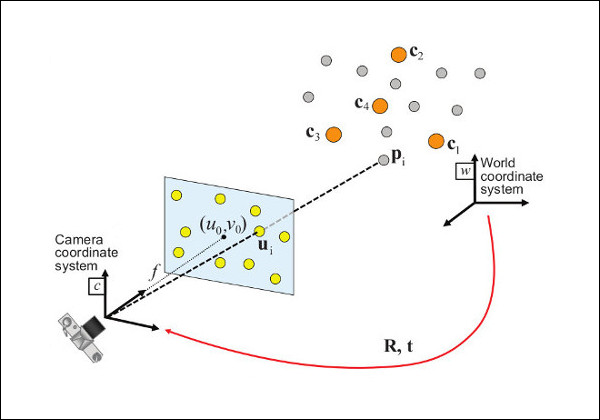
\includegraphics[width=140mm]{figures/pnp}
  \caption{PnP problem. The pose of camera relative to the world coordinate}\label{fig:pnp_sample}
\end{figure}